\part{Introducción}

Una ataguía es una estructura temporal utilizada para drenar zonas cubiertas de agua, 
lo que permite construir en terrenos que, de otra forma, serían inaccesibles 
\citep{madanayaka2018}. Al diseñar una ataguía, es fundamental considerar diversos 
factores, como el caudal de infiltración, las presiones de poros, la estabilidad 
de la estructura y, sobre todo, la licuefacción y su factor de seguridad (FS).
 Este fenómeno ocurre cuando las presiones de poros alcanzan tal nivel que las 
 tensiones internas efectivas entre las partículas del suelo disminuyen, lo que provoca 
 que la mezcla de agua y sedimentos actúe como un fluido \citep{sumer2009}.
\\ \\
El presente proyecto tiene como objetivo el estudio y análisis de tres ataguías 
distintas, evaluando sus características mediante cálculos manuales a través de \textit{Python}, 
un \textit{solver} basado en diferencias finitas y un modelo a escala. De esta manera, se busca 
analizar la efectividad de cada método de análisis y realizar una comparación directa entre
 los resultados obtenidos.
\\ \\
En los cálculos manuales, se utilizó la Ley de Darcy, además de las ecuaciones necesarias
 para determinar una red de flujo teórica. De esta forma, se calcularon parámetros como el
  caudal de infiltración y la presión de poros a lo largo de toda la estructura.
\\ \\
Posteriormente, se desarrolló un \textit{solver} mediante diferencias finitas, un método numérico 
utilizado para calcular diferencias de potencial en grillas 2D o 3D \citep{zhang2005}. 
Así, al determinar que el flujo va de un potencial mayor a uno menor, fue posible obtener 
las redes de flujo y, con ello, los distintos parámetros necesarios.
\\ \\
Finalmente, se realizó un modelo a escala, en el que se simuló la ataguía y una falla
 por licuefacción. Además, se calibró el modelo computacional en base a los 
 datos obtenidos del modelo real, para determinar cuán efectivo es el cálculo numérico 
 en comparación con la realidad.
\\ \\
El modelo base utilizado a lo largo del informe es el siguiente:

\begin{figure}[H]
    \centering
    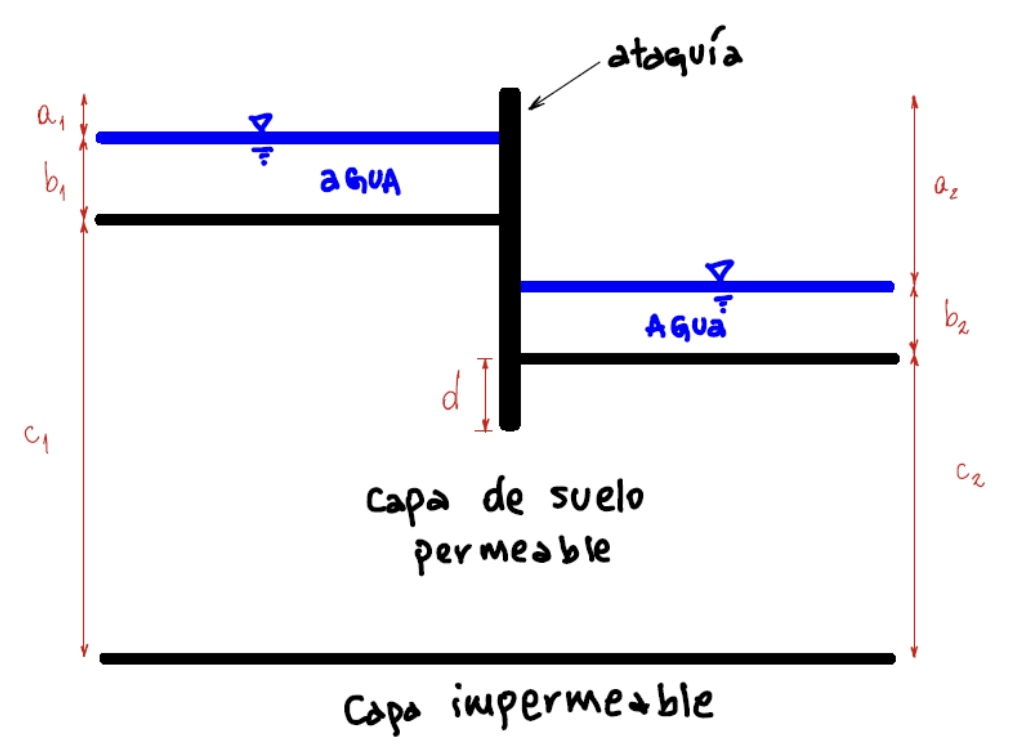
\includegraphics[width=0.45\textwidth]{FOTOS/modelo_base.png}
    \caption{Modelo base}
    Fuente: Guía de Proyecto
    \label{fig:modelo_base}
\end{figure}

Las medidas para los distintos casos se encuentran en la tabla \textbf{\ref{tab:medidas}}.
